%! suppress = MissingLabel
%! suppress = TooLargeSection
\documentclass[conference]{IEEEtran}
\IEEEoverridecommandlockouts


\usepackage{cite}
\usepackage{csquotes}
\usepackage{graphicx}
\usepackage{textcomp}
\usepackage{xcolor}
\usepackage{hyperref}
\usepackage{booktabs}

%! suppress = DiscouragedUseOfDef
\def\BibTeX{{%! suppress = PrimitiveStyle
\rm B\kern-.05em{%! suppress = PrimitiveStyle
\sc i\kern-.025em b}\kern-.08em
T\kern-.1667em\lower.7ex\hbox{E}\kern-.125emX}}

\begin{document}
\title{'Cloud testing tools for small to medium applications'}

\author{
	\IEEEauthorblockN{1
		\textsuperscript{st} Bachmann Lucius
	}
	\IEEEauthorblockA{
		\textit{Department of Informatics} \\
		\textit{University of Zurich}\\
		Zurich, Switzerland \\
		lucius.bachmann@gmx.ch
	}
}

\maketitle

\begin{abstract}
	Cloud computing is pervasive in the software industry.
With the advancement of web technology it is now possible to fulfill most of the computing needs as a service
in the cloud.
The services offering cloud services are also using other cloud services to perform their computing.
The development effort to develop and deploy an application to the cloud becomes less every year.
This also allows to use testing tools in the cloud to speed up the development and reduce cost for the development.
The following paragraphs will show how small to medium sized applications can leverage the cloud to test their application.

\end{abstract}

\begin{IEEEkeywords}
	cloud, test, github actions, cypress
\end{IEEEkeywords}

\section{Introduction}

Using the cloud offers many opportunities for entities offering or consuming services over the internet.
According to NIST \enquote{Cloud computing is a model for enabling ubiquitous, convenient, on-demand network access to a shared
	pool of configurable computing resources (e.g., networks, servers, storage, applications, and services) that
	can be rapidly provisioned and released with minimal management effort or service provider interaction.}\cite{mell2011nist}.
Not having to estimate the infrastructure needs upfront, not having to pay for resources not needed, not needing to maintain
the hardware, operating system, or even the application gives developers the possibility to devote more time and money
to delivering value.
Cloud computing can not only be used to deliver a service with an application but also in the development process of
the application itself.
Cloud services can be used for version control, review, build, testing, delivery, and deployment of the application.
These cloud testing techniques can not only be used for large-scale distributed systems, but they can also reduce the
effort and costs for testing small to medium-sized applications.
How these cloud testing techniques can be applied to a small to medium-sized application will be shown through the example
of eCampV3, an open-source web application to plan camps for various organizations.
The next paragraphs will be structured as follows:
In the remaining part of the introduction, some technological terms will be introduced, and the eCampV3 application will be
outlined.
Then follows the Related Work chapter where the research is presented, which describes the cloud testing tools that
will be used in the experiment.
The Method chapter then describes how the experiment was planned.
Then follows the Experiment section, which describes how these cloud testing tools can be applied.
The last chapter summarizes the findings and outlines possible future research.

\subsection{Technological terms}

\subsubsection{OCI containers and docker}

The Open Container Initiative (OCI) is a project to create standards around containers\cite{oci-website}.
Containers are a way to package (image spec), distribute (distribution spec), and run (runtime spec) an application
which may consist of binaries or a script with its interpreter.
The application can be shipped with all its dependencies so that the runtime does not need to adhere to any
requirements except for the runtime spec.
But a container is not a virtual machine with all its drawbacks; the kernel of a container is shared with the host system.
Thus, the image of a container can be smaller, and running the container usually requires fewer resources than running the same application
in a virtual machine.
Docker Inc.\ offers one implementation of the OCI specifications with a build tool for OCI images (buildkit), a runtime (containerd),
and a CLI (docker-cli) to interact with the build tool and the runtime\cite{docker-container-runtime-website}.

\subsubsection{Kubernetes}

Kubernetes is a tool developed and open-sourced by Google to manage and orchestrate multiple containers\cite{kubernetes-docs}.
It allows you to configure which containers should run, under which port a container is accessible,
how the containers can interact with each other, under which conditions a container is considered healthy, and it also allows
you to inject configuration files, environment variables, and secrets into the container\cite{kubernetes-docs}.
With the configuration, the user describes the state in which the cluster should be, and Kubernetes then performs the
operations like starting a container, configuring the network, or injecting configuration to reach this state\cite{kubernetes-docs}.
If a container crashes and the cluster deviates from the configured state, Kubernetes can automatically detect that
the state has deviated and then tries to restore the desired state by, for example, restarting a container\cite{kubernetes-docs}.
Kubernetes can also be used on multiple nodes, where one main node can deploy the containers to many child nodes,
thus providing an easy way for horizontal scaling\cite{kubernetes-docs}.

\subsubsection{Helm}

Helm is a package manager for Kubernetes\cite{helm-website}.
A collection of Kubernetes configuration files can be packaged together and published as a Helm chart on a repository
like artifacthub.io\cite{artifacthub-io}.
Helm also offers the possibility to use templates for your Kubernetes configuration files so that the Helm chart
can be adapted when it's deployed to a Kubernetes cluster.

\subsubsection{Github Actions}

GitHub Actions is a CI/CD service offered by GitHub\cite{github-actions-website}.
It allows you to configure workflows with YAML that integrate well with the version control, review,
and issue tracking system of GitHub itself.
A workflow consists of trigger events like a git push to a branch, a pull request, a manual workflow dispatch, or
other triggers and jobs.
In each job, different steps can be defined to build, test, or deploy a service.
An example of such a workflow can be found at the following link: \href{https://github.com/ecamp/ecamp3/blob/7a1cf92e3eee27b0b942fcd87bd8ce5c221089b7/.github/workflows/reusable-build-and-push.yml}{ecamp3/reusable-build-and-push.yml}.
For each job, a virtual machine is provisioned in which this job is executed\cite{github-actions-about-runner}.

\subsection{eCamp Version 3}

eCamp is a web application designed to help organize camps for youth organizations like the
scouts, YMCA (Young Men Christian Organization)\cite{ymca-website}, YWCA, or the Jubla.
It allows for collaborative scheduling of activities during the camp and detailed planning
according to the regulations of the Swiss federal support program for sport activities (Y+S) with young people\cite{J+S-Website,ecamp3-website}.
eCamp version 2 has been live since at least 2010\cite{ecamp2-first-commit} and has already been used to plan numerous camps.
The new version 3 has been in development for 5 years\cite{ecamp3-website} with the goal of separating frontend and backend,
and leveraging known, active, and newer frameworks for frontend and backend for bug fixes, security improvements,
and new features to enhance the usability, accessibility, and maintainability of the application.

\subsubsection{Architecture}

The application uses 5 components depicted in Figure\ref{fig:ecamp3-architecture}.
The frontend is a Vue application bundled with Vite and served by an NGINX web server.
The API is a PHP application using the API Platform framework, which is also served by a web server.
The print service is a Nuxt application that triggers the browserless container to fetch a printable HTML of a single activity
or a whole camp from the print service, and then convert it to a PDF\@.
The PDF is then served back to the frontend.

\begin{figure}[h!]
	\centering
	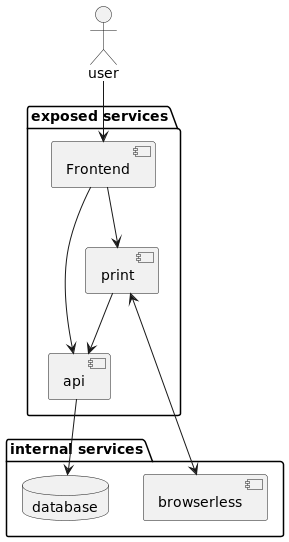
\includegraphics[height=\columnwidth]{sections/assets/ecamp3-architecture}
	\caption{eCamp V3 Architecture}
	\label{fig:ecamp3-architecture}
\end{figure}

\subsubsection{Deployment}

The application is currently deployed to a Kubernetes cluster on DigitalOcean.
As the database, a managed Postgres instance is used, which already includes scalability and backups for 5 days.
To separate the stages, 3 clusters are used for development, staging, and production.
For all self-developed services, the respective applications are packaged with Docker in an OCI image and then
pushed to Docker Hub using GitHub Actions\cite{ecamp3-reusable-build-and-push}.
These images are then deployed to the respective Kubernetes cluster using a Helm chart\cite{ecamp3-reusable-dev-deployment, ecamp3-deployment-stage-prod}.

\section{Related work}

\enquote{A Systematic Review on Cloud Testing} conducted a literature review using the guidelines for systematic reviews in software engineering research\cite{bertolino2019systematic}.
They analyzed 147 publications between 2012 and 2017 after excluding 632 publications\cite{bertolino2019systematic}.
The publications could be categorized into \enquote{Testing in the Cloud (TiC)}, \enquote{Testing of the Cloud (ToC)}, and their combination \enquote{Testing of the Cloud in the Cloud (Toic)}\cite{bertolino2019systematic}.
The most investigated area was test execution, followed by the test objectives, which comprised of performance, functional, security, reliability, and elasticity\cite{bertolino2019systematic}.
In the conclusion, they highlighted the ElasTest project, which aims to improve the efficiency and effectiveness of the testing process of large software systems by leveraging the potential of the cloud\cite{bertolino2019systematic, bertolino2020cloud}.

\enquote{A Survey of Software Testing in the Cloud} also conducted a literature review on publications between 2009 and 2012.
They categorized the publications into \enquote{Testing the Cloud-resident Applications}, which can be described as ToC,
\enquote{Providing Testing Software as Services in the Cloud}, which can be described as TiC, and both combined (ToiC).
They also divided the papers along the test level (Acceptance Testing, System Testing, Unit Testing, and Integration Testing)
and the test type (Functional Testing, Performance Testing, Security Testing, and Interoperability Testing) and concluded that a research gap exists in the Acceptance test level and the Interoperability test type\cite{6258440}.

\enquote{Cloud Testing Automation: Industrial Needs and ElasTest Response} conducted an empirical study comparing
testing teams using ElasTest and teams not using ElasTest on the same system under test.
The study was conducted on four different applications, each developed by a different institution or company,
with a testing team pair for each application.
The tool ElasTest was still under development when the study was conducted and not yet feature complete.
They received mixed results regarding the key performance indicators from the four different testing team pairs, but
concluded that cloud testing may bring some advantages in terms of scalability and reusability\cite{bertolino2020cloud}.

\enquote{Modern Web Automation with Cypress.io} evaluated Cypress.io\cite{cypress-website} as a tool to write and run end-to-end tests
against a web application\cite{jyolsna2022modern}.
Cypress.io was proposed as an alternative to existing end-to-end test automation frameworks like record and replay
frameworks\cite{jyolsna2022modern}.
The paper describes how Cypress was used to write the end-to-end tests for a Smart TV application.
They concluded that Cypress was a mature test automation tool that allowed writing the tests during
the development of the application\cite{jyolsna2022modern}.
The tests were stable and fast, the test scripts were simple to read and extend, and the standard web development tools
provided by the browser could be used for debugging, making test debugging simpler\cite{jyolsna2022modern}.

\enquote{Evaluation of Cloud-Based Performance Testing for Online Shopping Websites} highlighted the importance of
performance testing for online shopping applications.
During offers or holiday sales, online shopping applications often experience sudden traffic bursts.
However, it is crucial for them to remain available and responsive during such peak periods.
Performance tests can simulate the load, even against a separate instance, and help identify performance bottlenecks
before the application crashes in production.
The authors described three tools: Apache JMeter, Load Focus, and Nouvola, and conducted tests against three popular online
shopping applications in India - Flipkart, Snapdeal, and Amazon - using the Nouvola tool.

With the literature review, we have now identified the tools depicted in Table~\ref{tab:test-tools-and-frameworks}
for various test levels that can be used to test cloud applications.

\begin{table}[h]
	\centering
	\begin{tabular}{| l | l | l |}
		\toprule
		\textbf{Tool}                            & \textbf{Level} & \textbf{Type} \\
		\midrule
		ElasTest\cite{bertolino2019systematic}   & Acceptance     & Functional    \\
		                                         & System         & Performance   \\
		                                         &                & Security      \\
		\midrule
		Apache JMeter\cite{janani2015evaluation} & System         & Performance   \\
		\midrule
		Cypress\cite{mobaraya2019technical}      & System / Unit  & Functional    \\
		\midrule
	\end{tabular}
	\caption{Test tools and frameworks}
	\label{tab:test-tools-and-frameworks}
\end{table}

\section{Method}
The literature review showcases various cloud testing tools that can be utilized for testing at different levels and for different types of testing.
Now it is possible to propose a concept on how these testing tools could be applied with TiC, ToC, or ToiC against the eCampV3 code base\cite{bertolino2019systematic}.
For each tool, the following questions can now be answered:
\begin{itemize}
	\item RQ1: How can these tools be applied?
	\item RQ2: Which test level and test type can be covered by this tool?
\end{itemize}
A third question would be: \enquote{Which bugs can be prevented by using this testing tool?}
The underlying research does not clearly indicate which types of bugs were prevented by using the respective tool, and
there is not enough data available about the development process and bugs in production of eCampV3 to answer this question.
Table~\ref{tab:test-levels-and-tools} illustrates the different tools for which the experiment tries to describe
how the tools can be applied to perform the different levels and types of tests.

\begin{table*}[t]
	\centering
	\begin{tabular}{| l | l | l |}
		\toprule
		\textbf{Level} & \textbf{Type} & \textbf{Tool}                                \\
		\midrule
		Unit           & Functional    & Github Actions + test runner                 \\
		               & Performance   & Github Actions + test runner                 \\
		\midrule
		UI Component   & Functional    & Github Actions + test runner + mock renderer \\
		               & Performance   & Github Actions + test runner + mock renderer \\
		\midrule
		Integration    & Functional    & Github Actions + test runner                 \\
		               & Performance   & Github Actions + test runner                 \\
		               & Security      & Github Actions + test runner                 \\
		\midrule
		System         & Functional    & Github Actions + Cypress, ElasTest           \\
		               & Performance   & Apache JMeter, ElasTest                      \\
		               & Security      & ElasTest                                     \\
		               & Acceptance    & Github Actions + Cypress, ElasTest           \\
		\midrule
	\end{tabular}
	\caption{Test types, levels and tools}
	\label{tab:test-levels-and-tools}
\end{table*}

\section{Experiment}
\subsection{Github Actions + test runner + mock renderer}
For the different services in use, setting up GitHub Actions and the language and framework-specific test runner can be done by following the documentation.
This has already been done for the eCampV3 application.\newline
For the API, the following components are needed:
\begin{itemize}
	\item Dependencies: \href{https://github.com/ecamp/ecamp3/blob/7a1cf92e3eee27b0b942fcd87bd8ce5c221089b7/api/composer.json}{api/composer.json}
	      \subitem The dependencies for the framework api-platform
	      \subitem phpunit/phpunit
	      \subitem symfony/phpunit-bridge
	\item Configuration for the class loader: \href{https://github.com/ecamp/ecamp3/blob/7a1cf92e3eee27b0b942fcd87bd8ce5c221089b7/api/composer.json\#L88}{api/composer.json\#88}
	\item The script to run tests: \href{https://github.com/ecamp/ecamp3/blob/7a1cf92e3eee27b0b942fcd87bd8ce5c221089b7/api/composer.json\#L110}{api/composer.json\#110}
	\item A PHPUnit configuration: \href{https://github.com/ecamp/ecamp3/blob/7a1cf92e3eee27b0b942fcd87bd8ce5c221089b7/api/phpunit.xml.dist}{api/phpunit.xml.dist}
	\item A job in the GitHub Actions: \href{https://github.com/ecamp/ecamp3/blob/7a1cf92e3eee27b0b942fcd87bd8ce5c221089b7/.github/workflows/continuous-integration.yml#L111,L182}{continuous-integration.yml\#L111,L182}
	      \subitem with the database for the integration tests: \href{https://github.com/ecamp/ecamp3/blob/7a1cf92e3eee27b0b942fcd87bd8ce5c221089b7/.github/workflows/continuous-integration.yml#L117,L130}{continuous-integration.yml\#L117,L130}
\end{itemize}

For the frontend, the following components are needed:
\begin{itemize}
	\item Dependencies: \href{https://github.com/ecamp/ecamp3/blob/7a1cf92e3eee27b0b942fcd87bd8ce5c221089b7/frontend/package.json}{frontend/package.json}
	      \subitem @testing-library/jest-dom
	      \subitem @testing-library/user-event
	      \subitem @testing-library/vue
	      \subitem @vue/cli-plugin-unit-jest
	      \subitem @vue/cli-service
	      \subitem @vue/test-utils
	      \subitem @vue/vue2-jest
	      \subitem jest-canvas-mock
	      \subitem jest-serializer-vue-tjw
	\item A test script: \href{https://github.com/ecamp/ecamp3/blob/7a1cf92e3eee27b0b942fcd87bd8ce5c221089b7/frontend/package.json#L18,L20}{frontend/package.json\#L18,L20}
	\item Jest config: \href{https://github.com/ecamp/ecamp3/blob/7a1cf92e3eee27b0b942fcd87bd8ce5c221089b7/frontend/package.json#L175,L229}{frontend/package.json\#L175,L229}
	\item Configuration and context for the tests: \href{https://github.com/ecamp/ecamp3/tree/7a1cf92e3eee27b0b942fcd87bd8ce5c221089b7/frontend/.jest}{frontend/.jest}
	\item A job in the GitHub actions: \href{https://github.com/ecamp/ecamp3/blob/7a1cf92e3eee27b0b942fcd87bd8ce5c221089b7/.github/workflows/continuous-integration.yml#L184,L220}{continuous-integration.yml\#L184,L220}
\end{itemize}

For the print service, the following components are needed:
\begin{itemize}
	\item Dependencies: \href{https://github.com/ecamp/ecamp3/blob/7a1cf92e3eee27b0b942fcd87bd8ce5c221089b7/print/package.json}{print/package.json}
	      \subitem @vue/test-utils
	      \subitem babel-jest
	      \subitem jest
	      \subitem vue
	      \subitem vue-jest
	\item A test script: \href{https://github.com/ecamp/ecamp3/blob/7a1cf92e3eee27b0b942fcd87bd8ce5c221089b7/print/package.json#L18}{print/package.json\#L18}
	\item Jest config: \href{https://github.com/ecamp/ecamp3/blob/7a1cf92e3eee27b0b942fcd87bd8ce5c221089b7/print/package.json#L118,L139}{print/package.json\#L118,L139}
	\item A job in the GitHub actions: \href{https://github.com/ecamp/ecamp3/blob/7a1cf92e3eee27b0b942fcd87bd8ce5c221089b7/.github/workflows/continuous-integration.yml#L222,L260}{continuous-integration.yml\#L222,L260}
\end{itemize}

The testing tools themselves don't leverage the cloud, but running them in the GitHub actions allows the developers to
add and run tests without much effort.
Public repositories enjoy unlimited free GitHub action execution units on Linux runners\cite{github-actions-pricing},
and the developers do not have to reduce costs by selecting which tests should run on which stage.
The only thing slowing the developers down is the elapsed time of the tests and the time needed to maintain the job definitions and the tests.
The test runners used depend on the language and the framework.
Other test runners can also be used, for example, Jest\cite{jest-website} could be replaced with vitest\cite{vitest-website}.
\newline
With this setup, it is now possible to write unit tests (\href{https://github.com/ecamp/ecamp3/blob/7a1cf92e3eee27b0b942fcd87bd8ce5c221089b7/common/helpers/__tests__/dateHelperUTCFormatted.spec.js}{dateHelperUTCFormatted.spec.js}),
integration tests (\href{https://github.com/ecamp/ecamp3/blob/7a1cf92e3eee27b0b942fcd87bd8ce5c221089b7/api/tests/Api/Camps/UpdateCampTest.php}{UpdateCampTest}),
and tests for UI components (\href{https://github.com/ecamp/ecamp3/blob/7a1cf92e3eee27b0b942fcd87bd8ce5c221089b7/frontend/src/components/form/base/__tests__/ESwitch.spec.js}{ESwitch.spec.js}).
Performance tests are also possible but limited to one node or thread acting on the class or function under test.
This can be useful if there is a critical part of the code that must be fast or gets called frequently.
If the performance degrades after a change, the code part leading to the performance decrease can be identified quickly.

With the help of the API platform framework, it is also possible to leverage the test runner to test certain security
aspects like access control lists, as can be seen in \href{https://github.com/ecamp/ecamp3/blob/7a1cf92e3eee27b0b942fcd87bd8ce5c221089b7/api/tests/Api/Camps/UpdateCampTest.php#L11,L100}{UpdateCampTest\#L11,L100}.

\subsection{Github Actions + Cypress}
Cypress uses Node.js to start a browser, which is installed on the host machine or in a container.
Currently, the following browsers are supported: Chrome, Chromium, Edge, Electron, and Firefox\cite{cypress-website-supported-browsers}.
Cypress then executes the test suites in this browser and generates screenshots and videos of the tests.

The following setup is needed to run Cypress tests:
\begin{itemize}
	\item Dependencies: \href{https://github.com/ecamp/ecamp3/blob/7a1cf92e3eee27b0b942fcd87bd8ce5c221089b7/e2e/package.json#L10}{e2e/package.json\#L10}
	      \subitem Cypress
	\item Browsers
	      \subitem In a container: \href{https://github.com/ecamp/ecamp3/blob/7a1cf92e3eee27b0b942fcd87bd8ce5c221089b7/docker-compose.yml#L158,L168}{docker-compose.yml\#L158,L168}
	      \subitem In GitHub Actions: \href{https://github.com/ecamp/ecamp3/blob/7a1cf92e3eee27b0b942fcd87bd8ce5c221089b7/.github/workflows/continuous-integration.yml#L352,L357}{.github/workflows/continuous-integration.yml\#L352,L357}
	\item A way to run the application: \href{https://github.com/ecamp/ecamp3/blob/7a1cf92e3eee27b0b942fcd87bd8ce5c221089b7/docker-compose.yml}{docker-compose.yml}
	\item Cypress configuration: \href{https://github.com/ecamp/ecamp3/blob/7a1cf92e3eee27b0b942fcd87bd8ce5c221089b7/e2e/cypress.config.js}{cypress.config.js}
	\item Tests: \href{https://github.com/ecamp/ecamp3/tree/7a1cf92e3eee27b0b942fcd87bd8ce5c221089b7/e2e/specs}{e2e/specs}
\end{itemize}
Cypress offers a GitHub action that allows you to run Cypress tests with minimal effort.
However, because this cannot be used locally, the eCamp team has decided to switch back to running the Cypress tests in
a container\cite{ecamp3-e2e-tests-in-container}.
This is also an example of how testing in the cloud makes it relatively easy to run tests.
Cypress does not offer abstractions for starting the services needed for end-to-end tests\cite{cypress-website-best-practice-web-servers},
so the setup of your application has to be executed by yourself, which is as complex as the application to test: \href{https://github.com/ecamp/ecamp3/blob/7a1cf92e3eee27b0b942fcd87bd8ce5c221089b7/.github/workflows/continuous-integration.yml#L262,L350}{.github/workflows/continuous-integration.yml\#L262,L350}.
\newline
Cypress can be used to perform functional and acceptance tests at the system level.
With the ability to leverage the cloud using GitHub Actions, achieving high coverage of functional and acceptance tests is possible.
If the elapsed time for end-to-end tests becomes too long, the tests can be divided into groups and run in parallel.
Even a possible future regression can be detected by the current end-to-end tests should it happen again.
This regression was introduced in the commit \href{https://github.com/ecamp/ecamp3/commit/55c728e5b543a920a97988882df2ea99136228ea}{fix(deps): update dependency nuxt to v2.16.0},
which included a breaking change with Tailwind CSS\@.
However, this was fixed by the pull request \href{https://github.com/ecamp/ecamp3/pull/3275}{fix(print): fixes tailwind/nuxt + e2e tests for print},
which addressed the issue and added tests to detect similar regressions in the future.

\subsection{Apache JMeter}
Apache JMeter is a Java application with a rich client GUI in Swing\cite{website-apache-jmeter}.
To automatically execute tests in the cloud using GitHub Actions, it is also possible to run an XML representation
of the test configuration called JMX. The setup for these tests involves three steps:
\begin{enumerate}
	\item Define a response time within which a defined percentile of the requests should be completed.
	\item Define a load at which the defined response time should be reached.
	\item Define a target against which the tests should be performed.
	\item Set up the GitHub Action to perform the job.
\end{enumerate}
eCampV3 is only in closed beta since the start of March 2023, so it's not known what load the application will be
under when most of the summer camps are in their busy planning phase.
The performance of the development setup using Docker Compose is not relevant to the end user, thus the target will
be an instance of eCampV3 deployed via Helm chart and running in a cluster.
If the load target can be handled by less than one Kubernetes node, it would be possible to run the tests against
the dev deployment, which already uses the latest commit on the devel branch and is deployed every 30 minutes.
Then, a test plan can be created using the Apache JMeter GUI and storing the configuration as a JMX file.
The apache-jmeter-action\cite{apache-jmeter-github-action} could then be used to run the tests.
If one GitHub Actions runner is not enough to generate the required load, a matrix build could be used to
start multiple GitHub Actions runners to generate the needed load.
\newline
With this setup, Apache JMeter could be used to perform performance tests.
However, setting up target deployments to perform the tests against may be costly and make the setup more involved.
Additionally, when performance degrades, it may be difficult to identify the root cause without additional tools.

\subsection{ElasTest}
ElasTest offers multiple ways to deploy the application.
The simplest way is to use their Docker image, which uses Docker outside of Docker\cite{medium-docker-outside-of-docker} (mounting the Docker socket into a container)
to start additional services\cite{elastest-docs-mini}.
However, the configuration of the projects, jobs, and systems under test is stored in a MySQL database.
So, if a new ElasTest instance is spun up for every execution of the continuous integration pipeline,
it needs to be seeded with the project configuration.
Therefore, a more involved setup is needed where ElasTest runs independently of GitHub Actions and can be used to run tests triggered by either GitHub Actions or manually.
ElasTest offers documentation to deploy it to a virtual machine using a template file for Amazon AWS\cite{elastest-docs-aws}.
The next option is to use Kubernetes, where they offer Kubernetes manifests\cite{elastest-docs-kubernetes}.
Since eCampV3 already uses Kubernetes and has clusters running on DigitalOcean, the second option seems feasible.
The first step would be to convert the Kubernetes manifests provided by ElasTest at \href{https://github.com/elastest/elastest-toolbox/tree/b8cd58c3061b10f018824efbffcb9ed88a3e2ef0/kubernetes/ek}{elastest-toolbox/kubernetes/ek}
to a Helm chart so that the different files can be easily applied and the configuration of the cluster can be changed without modifying the tracked manifest files.
To avoid users needing to use port forwarding to access ElasTest, an ingress with some form of authentication
(such as Basic Auth\cite{kubernetes-basic-auth-ingress}, Oauth2Proxy\cite{github-oauth2-proxy}, or KeyCloak\cite{keycloak-kubernetes}) could be added.
\newline
Then ElasTest could be used to perform end-to-end, security, or performance tests against either the eCampV3 application deployed with Docker Compose or against
an instance running in a Kubernetes cluster.
For end-to-end tests, ElasTest uses Selenium under the hood, simplifying the process of spinning up a browser and connecting it with the test.
For security tests, ElasTest's Security Service uses ZAP from OWASP\cite{website-owasp-zap, elastest-code-ess-dockerfile}.
Therefore, performing security tests with ZAP could be achieved by using the image provided by OWASP directly and omitting
the overhead of setting up and maintaining ElasTest.
We couldn't find information on how performance testing would be conducted with ElasTest and how ElasTest would simplify that process.
\newline
This approach with a central instance also has its drawbacks.
Currently, most of the GitHub actions can be changed in a pull request, and the changed workflow is then used
for the GitHub action runs and thus tested.
With a centralized configuration in a separate ElasTest instance, every change in the test configuration has to either
be applied to all branches simultaneously or requires a migration of the test configuration.

\section{Conclusion}

The literature review showed that there are many tools available to fulfill most of the requirements for cloud testing.
The experiment demonstrated how these tools can be applied to test a specific test type at a certain test level,
and most of them can be set up with reasonable effort.
However, for performance testing, the setup effort increases when testing with big loads.
ElasTest stands out compared to other tools in terms of setup effort and design choice.
It uses a centralized configuration stored in a MySQL database instead of relying on a text representation (e.g., YAML, XML, scripts)
that can be put under version control, which may impact the efficiency of managing and configuring tests for different branches.
ElasTest has promising features such as log aggregation and integration with OWASP ZAP for security scanning
The question of the benefits of applying a testing tool could not be answered.
More data is needed on which bugs can be prevented by implementing test types at different levels in applications of varying sizes and complexities.
Future work could involve performing similar analyses on different applications using different cloud testing tools to gather more data.
With this data developers can then decide if they need to test for certain bugs, at which level they want to test
for them and with which tool they can achieve this goal efficiently.
Additionally, static code analysis tools should be included in the research, as they may detect certain bugs without executing code,
potentially resulting in less execution time and lower setup and maintenance costs.

\bibliographystyle{IEEEtran}
\bibliography{main}

\date{\today}



\newpage
%
\end{document}